%
% Main document
% ===========================================================================
% This is part of the document "Project documentation template".
% Authors: brd3
%

% Document informations
%---------------------------------------------------------------------------
\def \module		{Modul xyz}									% Module name
\def \title			{Template fuer Scripte}			% Title
\def \version		{1.0}
\def \author		{rct1}
%---------------------------------------------------------------------------

%---------------------------------------------------------------------------
\documentclass[
	a4paper,					% paper format
	10pt,							% fontsize
%	twoside,					% double-sided
	oneside,					% one-sided
	openright,				% begin new chapter on right side
	notitlepage,			% use no standard title page
	parskip=half,			% set paragraph skip to half of a line
]{scrreprt}					% KOMA-script report
%---------------------------------------------------------------------------

\raggedbottom
\KOMAoptions{cleardoublepage=plain}			% Add header and footer on blank pages


% Load Standard Packages:
%---------------------------------------------------------------------------
\usepackage[standard-baselineskips]{cmbright}

\usepackage[ngerman]{babel}							% german hyphenation
%\usepackage[latin1]{inputenc}  				% Unix/Linux - load extended character set (ISO 8859-1)
\usepackage[ansinew]{inputenc}  				% Windows - load extended character set (ISO 8859-1)
\usepackage[T1]{fontenc}								% hyphenation of words with ä,ö and ü
\usepackage{textcomp}										% additional symbols
\usepackage{ae}													% better resolution of Type1-Fonts 
\usepackage{fancyhdr}										% simple manipulation of header and footer 
\usepackage{graphicx}                   % integration of images
\usepackage{float}											% floating objects
\usepackage{caption}										% for captions of figures and tables
\usepackage{booktabs}										% package for nicer tables
\usepackage{tocvsec2}										% provides means of controlling the sectional numbering
\usepackage{rotating}										% rotating tables and other objects
\usepackage{pdflscape}									% change single pages landscape
\usepackage{tabularx}										% create nice tables
\usepackage{pdfpages}										% insert full pdf pages
\usepackage{nameref}										% reference by name, not by chapter number
\usepackage{dirtree}										% create directory trees
\usepackage{listings}										% include source code
%---------------------------------------------------------------------------

% Load Math Packages
%---------------------------------------------------------------------------
\usepackage{amsmath}                    % various features to facilitate writing math formulas
\usepackage{amsthm}                     % enhanced version of latex's newtheorem
\usepackage{amsfonts}                   % set of miscellaneous TeX fonts that augment the standard CM
\usepackage{amssymb}										% mathematical special characters
\usepackage{exscale}										% mathematical size corresponds to textsize
%---------------------------------------------------------------------------

% Package to facilitate placement of boxes at absolute positions
%---------------------------------------------------------------------------
\usepackage[absolute]{textpos}
\setlength{\TPHorizModule}{1mm}
\setlength{\TPVertModule}{1mm}
%---------------------------------------------------------------------------					
			
% Definition of Colors
%---------------------------------------------------------------------------
\RequirePackage{color}													% Color (not xcolor!)
\definecolor{linkblue}{rgb}{0,0,0.8}						% Standard
\definecolor{darkblue}{rgb}{0,0.08,0.45}				% Dark blue
\definecolor{brickred}{cmyk}{0,0.89,0.94,0.28}	% Brickred
%\definecolor{linkcolor}{rgb}{0,0,0.8}					% Blue for the web- and cd-version!
\definecolor{linkcolor}{rgb}{0,0,0}							% Black for the print-version!
\definecolor{bfhred}{rgb}{0.776,0,0.066}				% Red
\definecolor{codegray}{gray}{0.8}								% Source Code Gray
%---------------------------------------------------------------------------

% Hyperref Package (Create links in a pdf)
%---------------------------------------------------------------------------
\usepackage[
	pdftex,ngerman,bookmarks,plainpages=false,pdfpagelabels,
	backref = {false},										% No index backreference
	colorlinks = {true},                  % Color links in a PDF
	hypertexnames = {true},               % no failures "same page(i)"
	bookmarksopen = {true},               % opens the bar on the left side
	bookmarksopenlevel = {0},             % depth of opened bookmarks
	pdftitle = {\title},	   							% PDF-property
	pdfauthor = {\author},     					  % PDF-property
	pdfsubject = {\module},      				  % PDF-property
	linkcolor = {linkcolor},              % Color of Links
	citecolor = {linkcolor},              % Color of Cite-Links
	urlcolor = {linkcolor},               % Color of URLs
]{hyperref}
%---------------------------------------------------------------------------

% Set up page dimension
%---------------------------------------------------------------------------
\usepackage{geometry}
\geometry{
	a4paper,
	left=28mm,
	right=15mm,
	top=30mm,
	headheight=20mm,
	headsep=10mm,
	textheight=232mm,
	footskip=15mm
}
%---------------------------------------------------------------------------

% Makeindex Package
%---------------------------------------------------------------------------
\usepackage{makeidx}                    % To produce index
\makeindex                              % Index-Initialisation
%---------------------------------------------------------------------------

% Glossary Package
%---------------------------------------------------------------------------
% the glossaries package uses makeindex
% if you use TeXnicCenter do the following steps:
%  - Goto "Ausgabeprofile definieren" (ctrl + F7)
%  - Select the profile "LaTeX => PDF"
%  - Add in register "Nachbearbeitung" a new "Postprozessoren" point named Glossar
%  - Select makeindex.exe in the field "Anwendung" ( ..\MiKTeX x.x\miktex\bin\makeindex.exe )
%  - Add this [ -s "%tm.ist" -t "%tm.glg" -o "%tm.gls" "%tm.glo" ] in the field "Argumente"
%
% for futher informations go to http://ewus.de/tipp-1029.html
%---------------------------------------------------------------------------
\usepackage[nonumberlist]{glossaries}
\makeglossaries

\newglossaryentry{BibTeX}{name={BibTeX},description={Programm zur Erstellung von Literaturangaben und -verzeichnissen in \TeX- oder \LaTeX-Dokumenten}}
\newglossaryentry{StwVrz}{name={Stichwortverzeichnis},description={Verzeichnis mit Stichworten aus dem Text}}



%---------------------------------------------------------------------------

% Listings Package
%---------------------------------------------------------------------------
\lstdefinestyle{CCode}{
	showspaces=false,
	showtabs=false,
	language={[ANSI]C},
	breaklines=true,
	basicstyle={\footnotesize \ttfamily},
	backgroundcolor=\color{codegray},
	%frame=single,
	tab=\rightarrowfill,
	captionpos=b
}

\lstdefinestyle{CppCode}{
	showspaces=false,
	showtabs=false,
	language={[ISO]C++},
	breaklines=true,
	basicstyle={\footnotesize \ttfamily},
	backgroundcolor=\color{codegray},
	%frame=single,
	tab=\rightarrowfill,
	captionpos=b
}

\lstdefinestyle{JavaCode}{
	showspaces=false,
	showtabs=false,
	language={Java},
	breaklines=true,
	basicstyle={\footnotesize \ttfamily},
	backgroundcolor=\color{codegray},
	%frame=single,
	tab=\rightarrowfill,
	captionpos=b
}
%---------------------------------------------------------------------------

% Intro:
%---------------------------------------------------------------------------
\begin{document}                              	% Start Document
\settocdepth{section}														% Set depth of toc
\pagenumbering{roman}														
%---------------------------------------------------------------------------

% Set up header and footer
%---------------------------------------------------------------------------
\fancyhf{}																		% clean all fields
\fancypagestyle{plain}{												% new definition of plain style

% Use this for double-sided:
%	\fancyfoot[OL,ER]{\footnotesize							% footer left part -->	version
%		V\version \\
%		\author \\
%		\today
%	}
%	\fancyfoot[OR,EL]{\footnotesize \thepage} 	% footer right part --> page number
%	\fancyhead[OL,ER]{\module} 									% header right part --> module name
%	\fancyhead[OR,EL]{\footnotesize \leftmark}	% footer left part -->	chapter
%	\fancyhead[C]{															% header center part --> BFH logo
%		\begin{textblock}{0}[0,0](86,9)
%			
\includegraphics[scale=1.0]{Bilder/bfh_de_without_text.pdf}
%		\end{textblock}
%	}

% Use this for one-sided:
	\fancyfoot[L]{\footnotesize							% footer left part -->	version
		V\version \\
		\author \\
		\today
	}
	\fancyfoot[R]{\footnotesize \thepage} 	% footer right part --> page number
	\fancyhead[L]{\module} 									% header right part --> module name
	\fancyhead[R]{\footnotesize \leftmark}	% footer left part -->	chapter
	\fancyhead[C]{															% header center part --> BFH logo
		\begin{textblock}{0}[0,0](86,9)
			
\includegraphics[scale=1.0]{Bilder/bfh_de_without_text.pdf}
		\end{textblock}
	}
}

\renewcommand{\chaptermark}[1]{\markboth{\thechapter.  #1}{}}
\renewcommand{\headrulewidth}{0pt}				% no header stripline
\renewcommand{\footrulewidth}{0pt} 				% no bottom stripline

\pagestyle{plain}
%---------------------------------------------------------------------------


% Title Page and Abstract
%---------------------------------------------------------------------------

% Project documentation template
% ===========================================================================
% This is part of the document "Project documentation template".
% Authors: brd3
%

\begin{titlepage}


% BFH-Logo absolute placed at (29,10) on A4
% Actually not a realy satisfactory solution but working.
%---------------------------------------------------------------------------
\begin{textblock}{0}[0,0](29,10)
	\includegraphics[scale=1.0]{Bilder/BFH_Logo/\logo}
\end{textblock}

% Titel / Untertitel / Autor:
%---------------------------------------------------------------------------
\begin{flushleft}

\vspace*{2cm}

\fontsize{18pt}{20pt}\selectfont
Modul BTExxxx \\
\fontsize{12pt}{15pt}\selectfont\vspace{0.5em}
Fachbereich Elektro- und Kommunikationstechnik

\vspace{2cm}

\fontsize{30pt}{32pt}\selectfont 
\noindent \textcolor{titlecolor}{\textbf{\title}} \\

\vspace{10cm}
\fontsize{12pt}{15pt}\selectfont
\begin{tabbing}
xxxxxxxxxxxxxxxx\=xxxxxxxxxxxxxxxxxxxxxxxx	\kill
Author:			\> \author					\\
Datum:			\> \today					\\
Version:		\> \version					\\
\end{tabbing}
\end{flushleft}

\vspace{1cm}
\fontsize{12pt}{15pt}\selectfont
Damit an der Berner Fachhochschule im Bereich der technischen Informatik Module abgehalten werden k�nnen, braucht es im Normalfall ein Skript. Da diese Skripte immer wieder �berarbeitet werden sollten, wird mit diesem Dokument eine Vorlage geliefert, welche das ganze auf \LaTeX{} aufbauend einheitlich macht.

\end{titlepage}

%
% ===========================================================================
% EOF
%

\cleardoubleemptypage
\setcounter{page}{1}
\chapter*{Vorwort}
\label{chap:vorwort}

In diesem Dokument soll einerseits kurz auf \LaTeX{} eingegangen werden, andererseits auf diese Vorlage.\\
Ein Dank geht dabei an David Burri, welcher das Bachelor-Thesis Template geschrieben hat, auf welchem dieses Dokument aufbaut. Es wurde lediglich noch ein bisschen erweitert und angepasst.

%---------------------------------------------------------------------------

% Table of contents and listings
%---------------------------------------------------------------------------
\tableofcontents
\listoffigures
\listoftables
\cleardoublepage
%---------------------------------------------------------------------------

\pagenumbering{arabic}

% Main part - Part I
%---------------------------------------------------------------------------
\part{Teil 1}
\label{part:teil1}
\onecolumn
\chapter{Einleitung}
\label{chap:teil1_einleitung}

Dieses Dokument dient einerseites zur Illustration der \LaTeX{} Vorlage anhand des Corporate Designs\index{Corporate Design} der Berner Fachhochschule\index{Berner Fachhochschule} und andererseits als Anleitung f�r deren Verwendung. Dabei wird vorausgesetzt, dass der Benutzer bereits Erfahrungen mit \LaTeX{} besitzt oder gewillt ist, sich w�hrend der Benutzung in das Thema einzuarbeiten. Im Quellenverzeichnis sind einige n�tzliche Eintr�ge zu diversen B�chern und Dokumenten im Internet �ber \LaTeX{} zu finden.

% Eintr�ge im Verzeichnis erscheinen lassen ohne hier eine Referenz einzuf�gen
\nocite{kopka:band1}
\nocite{raichle:bibtex_programmierung}
\nocite{MiKTeX}
\nocite{KOMA}
\nocite{TeXnicCenter}
\nocite{Marti06}
\nocite{Erbsland08}
\nocite{juergens:einfuehrung}
\nocite{juergens:fortgeschritten}


\section{Dokumentaufbau}
\label{sec:teil1_einleitung_aufbau}

Das vorliegende Dokument ist so aufgebaut wie die Dokumentation einer Projektarbeit oder Thesis\index{Thesis}. Im Kapitel \ref{chap:teil2_anleitungen} werden die verwendeten Pakete kurz erkl�rt und Hinweise gegeben, wie die Bibliographie und das Glossar zu verwenden sind. Kapitel \ref{chap:teil3_satzspiegeltest} stellt ein reines Beispielkapitel dar, um den Satzspiegel zu pr�fen.


\section{Kontakt}
\label{sec:teil1_einleitung_kontakt}

Die Hersteller dieser Vorlage sind nat�rlich froh um Verbesserungsvorschl�ge jeder Art.

\begin{table}[H]
	\centering
	\begin{tabular}{lll} \toprule
		\textbf{Vorname Name} & \textbf{E-Mail} & \textbf{Funktion} \\ \midrule
		Roger Weber & roger.weber@bfh.ch & Auftraggeber \\ \midrule
		David Burri & david.burri@bfh.ch & Erstellung der Bachelor-Thesis Vorlage \\ \midrule
		Tobias R�etschi & tobias.rueetschi@bfh.ch & Erstellung der Skript-Vorlage \\ \bottomrule
	\end{tabular}
	\caption{Kontaktpersonen}
	\label{tab:teil1_kontaktpersonen}
\end{table}


\section{Versions History}
\label{sec:teil1_einleitung_versionen}

Das Template wird ab und zu mal �berarbeitet. Daher ist es wichtig, die Versionskontrolle im Griff zu halten. Daher sollte folgende Tabelle immer weitergef�hrt werden.

\begin{table}[H]
	\centering
	\begin{tabular}{lll} \toprule
		\textbf{Version}	& \textbf{Datum}	& \textbf{Beschreibung}											\\ \midrule
		1.0					& 12. April 2013	& Template von BSc Thesis mit Anpassungen f�r ein Modul Script.	\\ \midrule
		1.1					& 19. Juli 2013		& BFH Logo durch neues ersetzt.									\\ \bottomrule
	\end{tabular}
	\caption{Versionshistory}
	\label{tab:teil1_versionen}
\end{table}


% Main part - Part II
%---------------------------------------------------------------------------
\part{Teil 2}
\label{part:teil2}
\onecolumn
\chapter{Anleitungen}
\label{chap:teil2_anleitungen}

Die nachfolgende Tabelle zeigt einige der wichtigsten Pakete\index{Paket}, die in der Bachelor-Thesis \LaTeX{} Vorlage verwendet werden.

\begin{table}[H]
	\centering
	\begin{tabular}{p{0.13\textwidth} p{0.75\textwidth}} \toprule
		\textbf{Paket} & \textbf{Funktion} \\ \midrule
		\texttt{cmbright}\index{cmbright} & Serifenlose Schriftart 'Computer Modern Bright' welche die Textcodierungen\index{Textcodierungen} OT1, T1 und TS1 unterst�tzt, sowie die mathematischen Zeichen wie auch die AMS Symbole \\ \midrule
		\texttt{ae} & Sorgt f�r besser aufgel�ste Schriften in PDF Dateien \\ \midrule
		\texttt{fancyhdr}\index{fancyhdr} & Einfache Anpassung der Kopf- und Fusszeilen \\ \midrule
		\texttt{graphicx}\index{graphicx} & Einbindung von Grafiken in \LaTeX{} dokumente \\ \midrule
		\texttt{booktabs}\index{booktabs} & Sch�nere Darstellung von Tabellen \\ \midrule
		\texttt{textpos}\index{textpos} & Vereinfachte absolute Positionierung von Boxen auf der Seite \\ \midrule
		\texttt{hyperref}\index{hyperref} & Paket zum Erstellen von Links in PDF Dateien \\ \midrule
		\texttt{geometry}\index{geometry} & Vereinfachte und verbesserte Anpassung des Standard-Satzspiegels \\ \midrule
		\texttt{makeidx}\index{makeidx} & Einfache Indexerstellung (siehe Kapitel \ref{sec:teil2_anleitungen_index})\\ \midrule
		\texttt{glossaries}\index{glossaries} & Erstellen von Glossaren (siehe Kapitel \ref{sec:teil2_anleitungen_glossar}) \\ \bottomrule
	\end{tabular}
	\caption{Pakete}
	\label{tab:teil2_pakete}
\end{table}

Die Tabelle \ref{tab:teil2_pakete_new} zeigt, welche Pakete zus�tzlich dazugekommen sind.

\begin{table}[H]
	\centering
	\begin{tabularx}{\textwidth}{|r|X|}
		\hline
		\textbf{Paket} & \textbf{Funktion} \\
		\hline
		\texttt{tabularx}	\index{tabularx}	& Paket um sch�ne Tabellen darzustellen																				\\
		\texttt{pdfpages}	\index{pdfpages}	& Einbinden von pdf-Dateien																										\\
		\texttt{nameref}	\index{nameref}		& Referenzieren per Name und nicht per Kapitelnummer (Darstellung der Links)	\\
		\texttt{dirtree}	\index{dirtree}		& Erstellen von Ordner-Datei-Strukturen																				\\
		\texttt{listings}	\index{listings}	& Paket zum darstellen von Source Code																				\\
		\hline
	\end{tabularx}
	\caption{Zus�tzliche Pakete}
	\label{tab:teil2_pakete_new}
\end{table}


\section{Stichwortverzeichnisse}
\label{sec:teil2_anleitungen_index}

\LaTeX{} ist in der Grundausstattung nicht f�hig ein \gls{StwVrz} \index{Stichwortverzeichnis} zu erstellen. Diese k�nnen in \LaTeX{} mit dem \texttt{makeidx} Paket und dem \texttt{makeindex}\index{makeindex} Programm erstellt werden. Die folgende Seite enth�lt eine ausf�hrliche Erkl�rung wie das Paket funktioniert und dessen Anwendung:

\begin{center}
	\url{http://de.wikibooks.org/wiki/LaTeX-W�rterbuch:_makeindex}
\end{center}

Grob zusammengefasst sind f�r ein Stichwortverzeichnis folgenden Punkte n�tig:

\begin{itemize}
	\item Einbinden des Paketes \texttt{makeidx}
	\item Durch den \texttt{\textbackslash makeindex} Befehl die Erstellung initialisieren
	\item Im Text laufend W�rter indexieren mit dem Befehl \texttt{\textbackslash index\{\}}
	\item Beim ersten Durchlauf der Dokumenterstellung wird das Verzeichnis erstellt und die mit \texttt{\textbackslash index\{\}} markierten Begriffe in der \texttt{.idx}-Datei gespeichert
	\item Beim zweiten Durchlauf wird die \texttt{.idx}-Datei sortiert, formatiert und als \texttt{.ind}-Datei abgespeichert, wobei \LaTeX{} nun die \texttt{.ind}-Datei in das Dokument einf�gt
\end{itemize}


\section{Glossar}
\label{sec:teil2_anleitungen_glossar}

Ein Glossar\index{Glossar} kann in \LaTeX{} ebenfalls mit dem \texttt{makeindex} Programm und dem \texttt{glossaries} Paket erstellt werden. Die folgende Auflistung zeigt das Vorgehen um ein Glossar zu erzeugen:

\begin{itemize}
	\item Einbinden des \texttt{glossaries} Pakets
	\item Falls es als sinnvoll erachtet wird, kann eine eigene Datenbank mit Glossareintr�gen erstellt werden. In dieser Vorlage wird mit einer solchen Datenbank gearbeitet, welche im Ordner \texttt{datenbanken} abgelegt ist. Eintr�ge aus der Datenbank werden nur in das Verzeichnis geschrieben, falls das Wort im Text auch wirklich vermerkt ist.
	\item Durch den \texttt{\textbackslash makeglossaries} Befehl wird die Erstellung initialisiert
	\item Neue Eintr�ge k�nnen mit dem Befehl \\ \texttt{\textbackslash newglossaryentry\{<ABK�RZUNG>\}\{name=\{<NAME>\},description=\{<BESCHRIEB>\}\}} \\ erstellt werden
	\item Im Text laufend W�rter referenzieren mit dem Befehl \texttt{\textbackslash gls\{<ABK�RZUNG>\}}
	\item �hnlich wie bei der Erstellung des Index, wird das Verzeichnis erst beim zweiten Durchlauf in das Dokument eingebunden
\end{itemize}

Damit das Ganze �berhaupt funktioniert, muss als Nachbearbeitung des Dokuments das Glossar mit \texttt{makeindex} erstellt werden. Dazu ist folgender Code in der Kommandozeile auszuf�hren:

\begin{center}
	\texttt{makeindex -s template.ist -t template.glg -o template.gls template.glo}
\end{center}

Bei den meisten \LaTeX -Editoren kann dies als Nachbearbeitungsschritt angegeben werden. Die nachfolgende Erkl�rung ist f�r das Programm TeXnicCenter. Unter dem Menupunkt \glqq Ausgabe\grqq{} -> \glqq Ausgabeprofile definieren\grqq{} (kurz: alt + F7) ist unter dem Register \glqq Nachbearbeitung\grqq{} das in Bild \ref{fig:teil2_nachbearbeitung} dargestellte Fenster zu finden. Anschliessend gilt es, einen neuen Eintrag einzuf�gen, wobei eine Anwendung wie auch ein Argument anzugeben ist. Die Anwendung ist in der MiKTeX Installation zu finden (\texttt{..\textbackslash MiKTeX X.X\textbackslash miktex\textbackslash bin\textbackslash makeindex.exe}). Als Argument ist die folgende Zeile eizutragen:

\begin{center}
	\texttt{-s \string"\%tm.ist\string" -t \string"\%tm.glg\string" -o \string"\%tm.gls\string" \string"\%tm.glo\string" }
\end{center}

\begin{figure}[H]
	\centering
	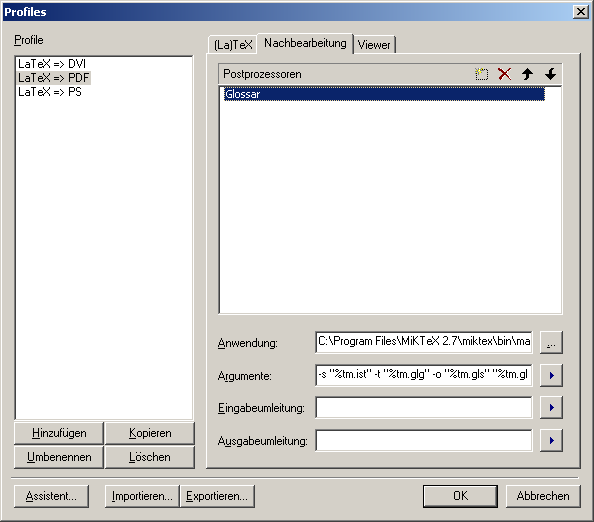
\includegraphics[scale=0.7]{bilder/profiles_glossar.png}
	\caption{Nachbearbeitung}
	\label{fig:teil2_nachbearbeitung}
\end{figure}


\section{Bibliographie}
\label{sec:teil2_anleitungen_bibliographie}

Zur Erstellung einer Bibliographie\index{Bibliographie} wird auf \gls{BibTeX} zur�ckgegriffen. Im Ordner \texttt{datenbanken} befindet sich eine \texttt{.bib}-Datei mit diversen Datenbankeintr�gen. Wie diese Eintr�ge zu erstellen sind, kann aus diversen Quellen im Internet oder in B�chern entnommen werden. Die Eintr�ge in der Datenbank werden nur dann in das Verzeichnis des Dokuments geschrieben, wenn die Quelle auch wirklich im Text zitiert wurde.

Unter den folgenden Adressen sind weitere Erl�uterungen zum Erstellen der Datenbank und deren Verwendung zu finden:
\begin{itemize}
	\item \url{http://en.wikipedia.org/wiki/BibTeX}
	\item \url{http://www.bibtex.org/de/}
\end{itemize}




% Main part - Part III
%---------------------------------------------------------------------------
\part{Teil 3}
\label{part:teil3}
\onecolumn
\chapter{Satzspiegeltest}
\label{chap:teil3_satzspiegeltest}

Weit hinten, hinter den Wortbergen, fern der L�nder Vokalien und Konsonantien leben die Blindtexte. Abgeschieden wohnen Sie in Buchstabhausen an der K�ste des Semantik, eines gro�en Sprachozeans. Ein kleines B�chlein namens Duden flie�t durch ihren Ort und versorgt sie mit den n�tigen Regelialien. Es ist ein paradiesmatisches Land, in dem einem gebratene Satzteile in den Mund fliegen. Nicht einmal von der allm�chtigen Interpunktion werden die Blindtexte beherrscht � ein geradezu unorthographisches Leben. Eines Tages aber beschlo� eine kleine Zeile Blindtext, ihr Name war Lorem Ipsum, hinaus zu gehen in die weite Grammatik.


\section{Der gro�e Oxmox}
\label{sec:teil3_satzspiegeltest_ombox}

Der gro�e Oxmox riet ihr davon ab, da es dort wimmele von b�sen Kommata, wilden Fragezeichen und hinterh�ltigen Semikoli, doch das Blindtextchen lie� sich nicht beirren. Es packte seine sieben Versalien, schob sich sein Initial in den G�rtel und machte sich auf den Weg. Als es die ersten H�gel des Kursivgebirges erklommen hatte, warf es einen letzten Blick zur�ck auf die Skyline seiner Heimatstadt Buchstabhausen, die Headline von Alphabetdorf und die Subline seiner eigenen Stra�e, der Zeilengasse. Wehm�tig lief ihm eine rethorische Frage �ber die Wange, dann setzte es seinen Weg fort. Unterwegs traf es eine Copy.

\begin{equation}
	\mathcal{N}(x \mid \mathbold{\mu}, \mathbold{\Sigma}) = \frac{1}{(2\pi)^{D/2}} \frac{1}{|\mathbold{\Sigma}|^{(1/2)}} \exp \left( -\frac{1}{2}(x-\mathbold{\mu})^{T}\mathbold{\Sigma}^{-1}(x-\mathbold{\mu}) \right)
\end{equation}

Die Copy warnte das Blindtextchen, da, wo sie herk�me w�re sie zigmal umgeschrieben worden und alles, was von ihrem Ursprung noch �brig w�re, sei das Wort \"und\" und das Blindtextchen solle umkehren und wieder in sein eigenes, sicheres Land zur�ckkehren. Doch alles Gutzureden konnte es nicht �berzeugen und so dauerte es nicht lange, bis ihm ein paar heimt�ckische Werbetexter auflauerten, es mit Longe und Parole betrunken machten und es dann in ihre Agentur schleppten, wo sie es f�r ihre Projekte wieder und wieder mi�brauchten. Und wenn es nicht umgeschrieben wurde, dann benutzen Sie es immernoch.


\section{Typoblindtext}
\label{sec:teil3_satzspiegeltest_typoblindtext}

Dies ist ein Typoblindtext. An ihm kann man sehen, ob alle Buchstaben da sind und wie sie aussehen. Manchmal benutzt man Worte wie Hamburgefonts, Rafgenduks oder Handgloves, um Schriften zu testen. Manchmal S�tze, die alle Buchstaben des Alphabets enthalten - man nennt diese S�tze \glqq Pangrams\grqq.

Sehr bekannt ist dieser: The quick brown fox jumps over the lazy old dog. Oft werden in Typoblindtexte auch fremdsprachige Satzteile eingebaut (AVAIL� and Wefox� are testing aussi la Kerning), um die Wirkung in anderen Sprachen zu testen. In Lateinisch sieht zum Beispiel fast jede Schrift gut aus.

\subsection{Demonstrandum}
\label{subsec:teil3_satzspiegeltest_typoblindtext_demonstrandum}

Quod erat demonstrandum. Seit 1975 fehlen in den meisten Testtexten die Zahlen, weswegen nach TypoGb. 204 � ab dem Jahr 2034 Zahlen in 86 der Texte zur Pflicht werden. Nichteinhaltung wird mit bis zu 245\texteuro oder 368\$ bestraft. Genauso wichtig in sind mittlerweile auch ��c��t�, die in neueren Schriften aber fast immer enthalten sind. Ein wichtiges aber schwierig zu integrierendes Feld sind OpenType-Funktionalit�ten. Je nach Software und Voreinstellungen k�nnen eingebaute Kapit�lchen, Kerning oder Ligaturen (sehr pfiffig) nicht richtig dargestellt werden.

\subsubsection{Subsubsection}
\label{subsubsec:teil3_satzspiegeltest_typoblindtext_demonstrandum_subsubsection1}

Dies ist ein Typoblindtext. An ihm kann man sehen, ob alle Buchstaben da sind und wie sie aussehen. Manchmal benutzt man Worte wie Hamburgefonts, Rafgenduks oder Handgloves, um Schriften zu testen. Manchmal S�tze, die alle Buchstaben des Alphabets enthalten - man nennt diese S�tze \glqq Pangrams\grqq. 

\subsubsection{Subsubsection}
\label{subsubsec:teil3_satzspiegeltest_typoblindtext_demonstrandum_subsubsection2}

Sehr bekannt ist dieser: The quick brown fox jumps over the lazy old dog. Oft werden in Typoblindtexte auch fremdsprachige Satzteile eingebaut (AVAIL� and Wefox� are testing aussi la Kerning), um die Wirkung in anderen Sprachen zu testen. In Lateinisch sieht zum Beispiel fast jede Schrift gut aus. Quod erat demonstrandum.


\section{Webstandards}
\label{sec:teil3_satzspiegeltest_webstandards}

�berall dieselbe alte Leier. Das Layout ist fertig, der Text l�sst auf sich warten. Damit das Layout nun nicht nackt im Raume steht und sich klein und leer vorkommt, springe ich ein: der Blindtext. Genau zu diesem Zwecke erschaffen, immer im Schatten meines gro�en Bruders \glqq Lorem Ipsum\grqq, freue ich mich jedes Mal, wenn Sie ein paar Zeilen lesen. Denn esse est percipi - Sein ist wahrgenommen werden.

Und weil Sie nun schon die G�te haben, mich ein paar weitere S�tze lang zu begleiten, m�chte ich diese Gelegenheit nutzen, Ihnen nicht nur als L�ckenf�ller zu dienen, sondern auf etwas hinzuweisen, das es ebenso verdient wahrgenommen zu werden: Webstandards n�mlich. Sehen Sie, Webstandards sind das Regelwerk, auf dem Webseiten aufbauen. So gibt es Regeln f�r HTML, CSS, JavaScript oder auch XML; Worte, die Sie vielleicht schon einmal von Ihrem Entwickler geh�rt haben. Diese Standards sorgen daf�r, dass alle Beteiligten aus einer Webseite den gr��ten Nutzen ziehen.

\begin{figure}[H]
	\centering
	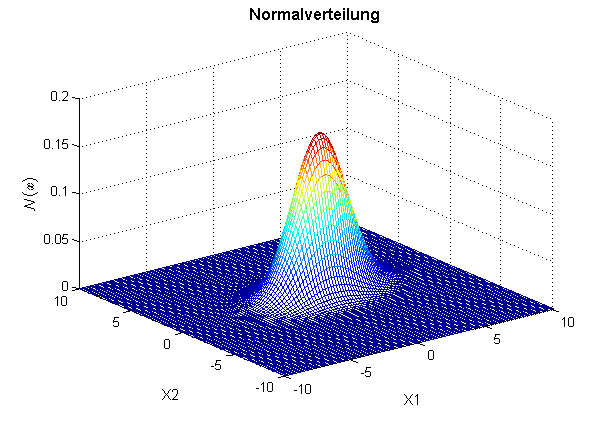
\includegraphics[scale=0.7]{bilder/multivariate_gauss.png}
	\caption{Normalverteilung}
	\label{fig:teil3_normalverteilung}
\end{figure}

Im Gegensatz zu fr�heren Webseiten m�ssen wir zum Beispiel nicht mehr zwei verschiedene Webseiten f�r den Internet Explorer und einen anderen Browser programmieren. Es reicht eine Seite, die - richtig angelegt - sowohl auf verschiedenen Browsern im Netz funktioniert, aber ebenso gut f�r den Ausdruck oder die Darstellung auf einem Handy geeignet ist. Wohlgemerkt: Eine Seite f�r alle Formate. Was f�r eine Erleichterung. Standards sparen Zeit bei den Entwicklungskosten und sorgen daf�r, dass sich Webseiten sp�ter leichter pflegen lassen. Nat�rlich nur dann, wenn sich alle an diese Standards halten.

\chapter{Source Code}
\label{chap:teil3_sourcecode}


\section{Direkte Eingabe des Source Code}

Im Listing \nameref{lst:teil3_c_code_beispiel} wird der C-Code in das Tex-File geschrieben.

\begin{lstlisting}[style=CCode, label=lst:teil3_c_code_beispiel, caption=C-Code Beispiel]
int main(int argc, void *argv) {
	boot();
	LED = 0xFF;
	shutdown();
	return 1;
}
\end{lstlisting}


\section{Einbinden des Source Code}

Im Listing \ref{lst:teil3_java_code_beispiel} wird ein Java-File direkt eingebunden.

\lstinputlisting[style=JavaCode, label=lst:teil3_java_code_beispiel, caption=Java-Code Beispiel]{SourceCode/JavaBeispiel.java}


% Attachment:
%---------------------------------------------------------------------------
\part{Anhang}
\label{part:anhang}
\onecolumn
\appendix
\settocdepth{section}
\chapter{Beliebiger Anhang}
\label{chap:bel_anhang}

Phasellus eget velit massa, sed faucibus nisi. Etiam tincidunt libero viverra lorem bibendum ut rutrum nisi volutpat. Donec non quam vitae lacus egestas suscipit at eu nisi. Maecenas non orci risus, at egestas tellus. Vivamus quis est pretium mauris fermentum consectetur. Cras non dolor vitae nulla molestie facilisis. Aliquam euismod nisl eget risus pretium non suscipit nulla feugiat. Nam in tortor sapien. Nam lectus nibh, laoreet eu ultrices nec, consequat nec sem. Nulla leo turpis, suscipit in vulputate a, dapibus molestie quam. Vestibulum pretium, purus sed suscipit tempus, turpis purus fermentum diam, id cursus enim mi a tortor. Proin imperdiet varius pellentesque. Nam congue, enim sit amet iaculis venenatis, dui neque ornare purus, laoreet porttitor nunc justo vel velit. Suspendisse potenti. Nulla facilisi.

\chapter{Weiterer Anhang}
\label{chap:anhang_B}

\section{Test 1}
Phasellus eget velit massa, sed faucibus nisi. Etiam tincidunt libero viverra lorem bibendum ut rutrum nisi volutpat. Donec non quam vitae lacus egestas suscipit at eu nisi. Maecenas non orci risus, at egestas tellus. Vivamus quis est pretium mauris fermentum consectetur. Cras non dolor vitae nulla molestie facilisis. Aliquam euismod nisl eget risus pretium non suscipit nulla feugiat. Nam in tortor sapien. 

\subsection{Umfeld}
Nam lectus nibh, laoreet eu ultrices nec, consequat nec sem. Nulla leo turpis, suscipit in vulputate a, dapibus molestie quam. Vestibulum pretium, purus sed suscipit tempus, turpis purus fermentum diam, id cursus enim mi a tortor. Proin imperdiet varius pellentesque. Nam congue, enim sit amet iaculis venenatis, dui neque ornare purus, laoreet porttitor nunc justo vel velit. Suspendisse potenti. Nulla facilisi.

%---------------------------------------------------------------------------

% Glossary
%---------------------------------------------------------------------------
\cleardoublepage
\phantomsection 
\addcontentsline{toc}{chapter}{Glossar}
\renewcommand{\glossaryname}{Glossar}
\printglossary
%---------------------------------------------------------------------------

% Bibliography
%---------------------------------------------------------------------------
\cleardoublepage
\phantomsection 
\addcontentsline{toc}{chapter}{Literaturverzeichnis}
\bibliographystyle{IEEEtranS}
\bibliography{Datenbanken/bibliography}{}
%---------------------------------------------------------------------------

% Index
%---------------------------------------------------------------------------
%\cleardoublepage
%\phantomsection 
%\addcontentsline{toc}{chapter}{Stichwortverzeichnis}
%\renewcommand{\indexname}{Stichwortverzeichnis}
%\printindex
%---------------------------------------------------------------------------

%---------------------------------------------------------------------------
\end{document}
